%set this to 0 to 
%set to zero to include figures, 10 or greater to exclude
%\count33=10
\count33=0
%
\chapter{Software Architecture}
\label{asf_chap}

The WRF Advanced Software Framework (ASF) implements the WRF software
architecture described in \citet{michalak99} and is the basis for the
WRF model, 3DVAR, and other components of the WRF system.  It provides
a common development platform meshing effort and experties of
geographically dispersed and institutionally diverse engineers and
scientists to bring WRF from a blank page to a fully-functional
modeling system in the short span of six years. 

Requirements include:

\begin{itemize}\setlength{\parskip}{-4pt}
  \item Community software
  \begin {itemize}
     \item Applicability across a range of applications
     \item Portability across a range of computing platforms
     \item Efficiency and scalability
     \item Single source code for maintainability
     \item Independent with respect to external packages
  \end {itemize}
  \item Support multiple dynamical cores and physics
  \item Nesting, moving nests
  \item Ability to interoperate within coupled modeling systems
\end{itemize}

\noindent
Various aspects of the WRF software design and implementation are
described in the next section. Because of their complexity, nesting and
I/O are described separately in sections that follow.


\section{WRF Advanced Software Framework}

The WRF ASF comprises a number of software layers and supporting
components: the Driver Layer, Mediation Layer, Model Layer, and a
meta-programming utility called the Registry.  By design, WRF is
package-neutral; the WRF ASF does not specify nor is it dependent upon
external packages for such things as interprocessor communication, data
formats, I/O, and coupling. Rather, the framework specifies that
package-specific instances of these functionalities be implemented
behind Application Program Interfaces (APIs), so that adapting a
particular package for use with WRF involves producing an
implementation of the API, without modification of the WRF software
itself.  API documents and other WRF software documentation are
available at \citep{sasi}.  The
benefits of the WRF ASF are facilitation of rapid development, ease of
extension, leverage of development effort by the WRF community at
large, software reuse, and ready adaptation to community model
infrastructure such as the Earth System Modeling Framework (ESMF).

%
% Figure 9.x
%
\ifnum\count33<9
\begin{figure}
  \centering
  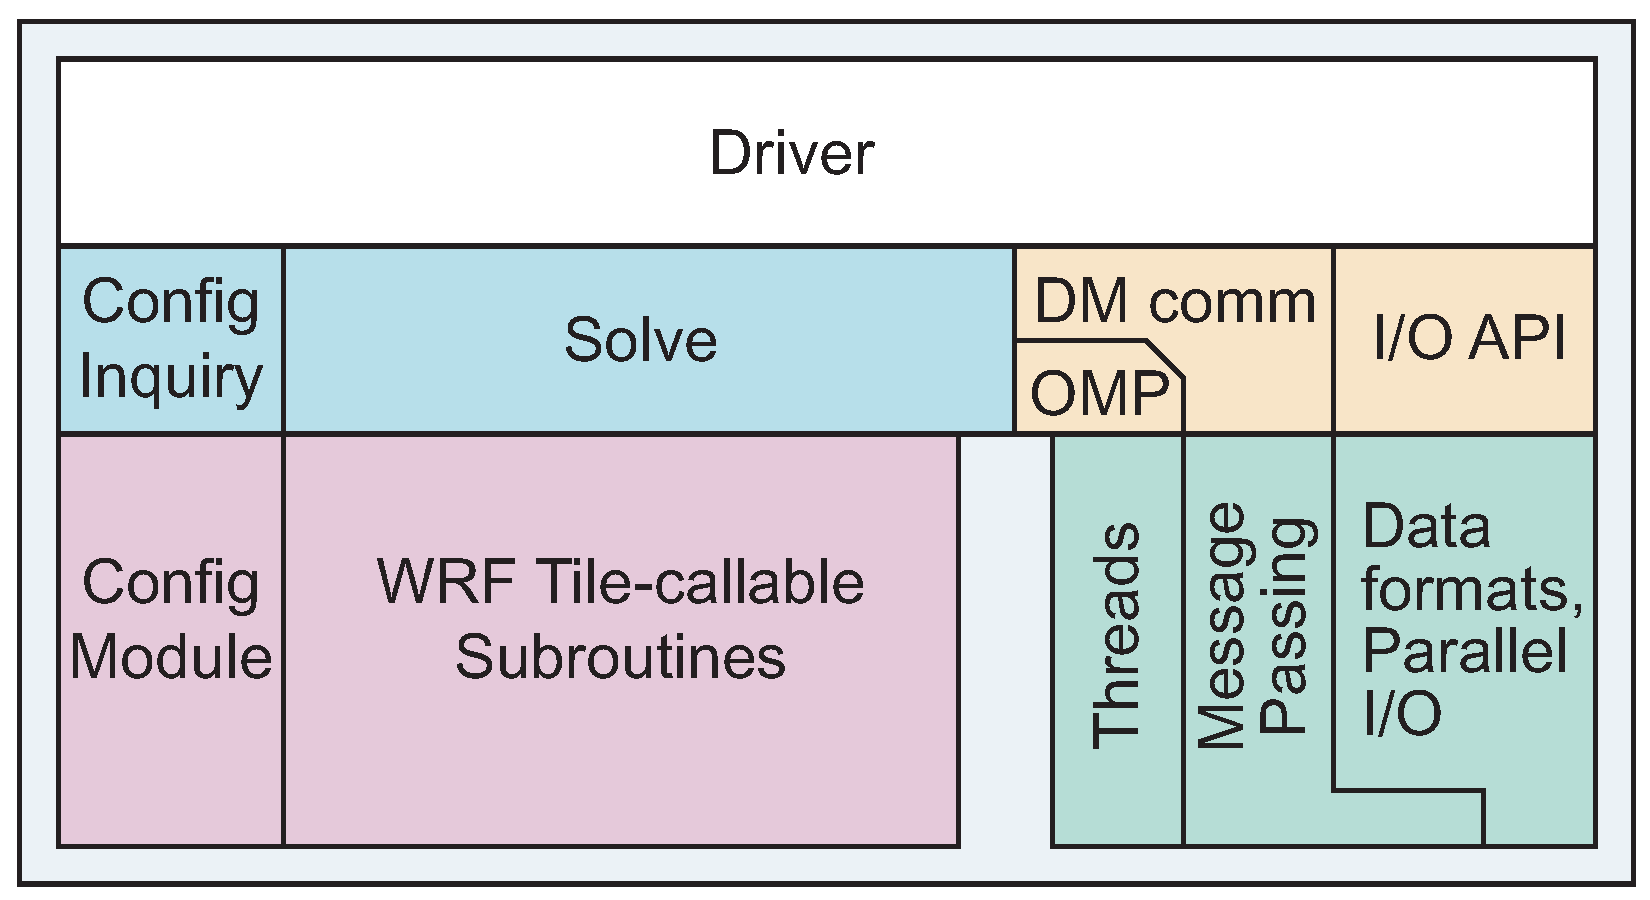
\includegraphics[width=6.5in]{figures/layout.pdf}
  \caption{\label{figure:5a}Layered WRF architecture.}
\end{figure}
\fi

\paragraph{The Driver Layer} 
handles run-time allocation and parallel decomposition
of model domain data structures; organization, management, interaction,
and control over nested domains, including the main time loop in the
model; high-level interfaces to I/O operations on model domains; and
the interface to other components when WRF is part of a larger coupled
system of applications.  Within the driver, each domain is represented
abstractly as a single object: a Fortran 90  derived data type containing
the dynamically allocated state data with pointers to other domains in
the nest hierarchy. Nesting is represented as a tree of domains rooted
at the top-level (most coarse resolution) domain. Each model time step
involves a recursive depth-first traversal over this tree, advancing
each node and its children forward to the next model time. Forcing,
feedback, and nest movement are also handled in the Driver.

\paragraph{The Mediation Layer} 
encompasses one time-step of a particular dynamical
core on a single model domain. Within this layer, the solve routine for
a dynamical core contains the complete set of calls to Model Layer
routines as well as invocation of interprocessor communication (halo
updates, parallel transposes, etc.) and multi-threading. The current
WRF implementation uses the RSL communication library
\citep{michalak00} that, in turn, uses the Message Passing Interface
(MPI) communication package.  Shared memory parallelism over tiles
-- a second level of domain decomposition within distributed
memory patches -- is also specified in the solve routines using
OpenMP.  

\paragraph{The Model Layer} 
comprises the actual computational routines that make
up the model:  advection, diffusion, physical parameterizations, and so
forth. Model layer subroutines are called through a standard Model
Layer Interface: all state data are passed as arguments, along with the
starting and ending indices in each of the three grid dimensions for
the tile that is being computed. Model layer subroutines may not
include I/O, stop statements, multi-threading, or interprocessor
communication, ensuring that they may be executed coherently for any
tile-decomposition or order of execution over tiles. The Model Layer
Interface is a contract between the ASF and the programmer/scientist
working at the Model Layer. Adherence to the interface ensures that a
Model Layer package incorporated into WRF will work on any parallel
computer to which the framework is ported. Model layer routines that
have horizontal data dependencies rely on the mediation layer to perform the
necessary interprocessor communication prior to their being called. The
programmer describes the communication type and pattern by adding an
entry to the Registry and then inserts a notation to perform the
communication at the appropriate location in the solve routine.

\paragraph{Data Structures.} \label{ds} The WRF ASF represents model
data structures differently at different layers.  In the higher levels
of the mediation layer and in the driver layer, above, operations are
on entire domains. Data representing the state of each domain are stored
as fields in a Fortran 90 derived data type that can be manipulated and
operated upon as a single entity.  Within and below the mediation
layer, operations are on individual data elements take place. Here,
each field appears individually as simple Fortran data type of between
zero and 5 dimensions.  Neither the WRF software architecture nor the
ASF specify {\em storage order} for multi-dimensional data but the WRF model itself
uses I-K-J. That is, the innermost stride-1 dimension is over I, then over
K; finally, J is outermost. This provides
the best compromise for efficient performance on both microprocessor and
vector systems \citep{michalak01}.

\paragraph{The Registry}\label{registry}
is a concise database of information about WRF data
structures and a mechanism for automatically generating large sections
of WRF code from the notations in the database.  The Registry database
is a collection of tables that lists and describes the WRF state
variables and arrays with their attributes such as dimensionality,
number of time levels, association with a particular dynamical core,
association with a particular physics package, membership in an input,
output, or restart dataset, communication operations on the data, information pertaining to nest forcing and feedback, and
some descriptive meta-data such as what the variable or array
represents and its units. From this database, the Registry generates
code for interfaces between layers of the infrastructure, packing and
unpacking code for communication and nesting, and field-by-field calls
to routines for model I/O -- code that would otherwise be extremely
time-consuming and error-prone to write and manage manually. 

The Registry also provides a very high-level interface for scientists
and other users to add or modify model state, configuration
information, I/O, and other key characteristics.  Adding or modifying a
state variable, simple array, or array of tracers in WRF is a matter of
modifying a line or two in the Registry.

Currently, the Registry automatically
generates 60-thousand of the total 250-thousand lines of WRF code.
A complete description and reference manual is available at \citep{sasi}.

\paragraph{Application Program Interfaces} 
(APIs) to external packages serve the important function of separating
code that is WRF from code that provides functionality that is needed
by WRF but that for various reasons is considered external,
interchangeable, or otherwise ``not-WRF.'' Reasons for considering
functionality external to WRF itself include user or institutional
preference, existing investment in a package, suitability for a
particular application, suitability for a particular computer platform,
preserving flexibility, leveraging external investment in a capability
and avoiding duplication of effort, and avoiding single points of
failure that come from relying too heavily on a single package.
Different packages that conform to the API specification can be swapped
in or out of a particular model configuration without changing WRF
itself.  Examples include packages for self-describing data formats
(e.g. NetCDF, HDF, and GRIB), interprocessor communication (RSL,
RSL\_LITE), model coupling toolkits and libraries (MCEL, MCT, ESMF).
Clean APIs also support reuse in the other direction; for example,
Earth System Modeling Framework developers are adapting the WRF I/O API
for use within the ESMF software.

Documentation for the WRF infrastructure, including reference
documentation for the Registry, the WRF I/O Application Program
Interface specification, and a web-based WRF code and documentation
browser (\citet{fiedler}) are maintained on-line at \citep{sasi}.
Additional software documentation for WRF is in-progress.


\paragraph{Parallelism.}
\label{asf_patch}
The WRF model is required to run efficiently on different types of
parallel machine. The WRF software architecture
addresses this issue by adopting a two-level decomposition for
parallelism in which domains may be decomposed into patches for
distributed memory; patches may, in turn, be multi-threaded over tiles
for shared memory (Figure \ref{figure:decomposition}). A patch is a
section of a model domain allocated to a single memory address space.
It may also include memory for halo regions, used to store data from
neighboring patches, or boundary regions, used to store data associated
with certain physical boundary conditions (e.g. periodic boundaries).
A tile is the amount of a patch that is allocated to one thread of
execution and every cell of a patch that requires computation must fall
into some tile. On a distributed memory machine with single-processor
nodes, there would be one patch per processor, each with a single tile.
On a distributed memory machine with multiple processors per node,
there would still be one patch per node (that is, per memory), but each
patch may contain a number tiles equal to or greater (perhaps much
greater) than the number of processors on each node.  Each domain in a
simulation may be decomposed and tiled independently.  This approach
addresses all current models for parallelism -- single-processor,
shared-memory, distributed-memory, and hybrid -- and also provides
adaptivity with respect to processor type: tiles may be sized and
shaped for cache-blocking or to preserve maximum vector length.

Particular decomposition, tiling strategies, and communication packages
are architecture- and application-specific and not part of the
WRF design.  The current implementation of WRF
uses two-sided MPI communication to handle exchanges between
patches and OpenMP to implement multithreading over tiles.

%
% Figure 9.x
%
\ifnum\count33<9
\begin{figure}
  \centering
  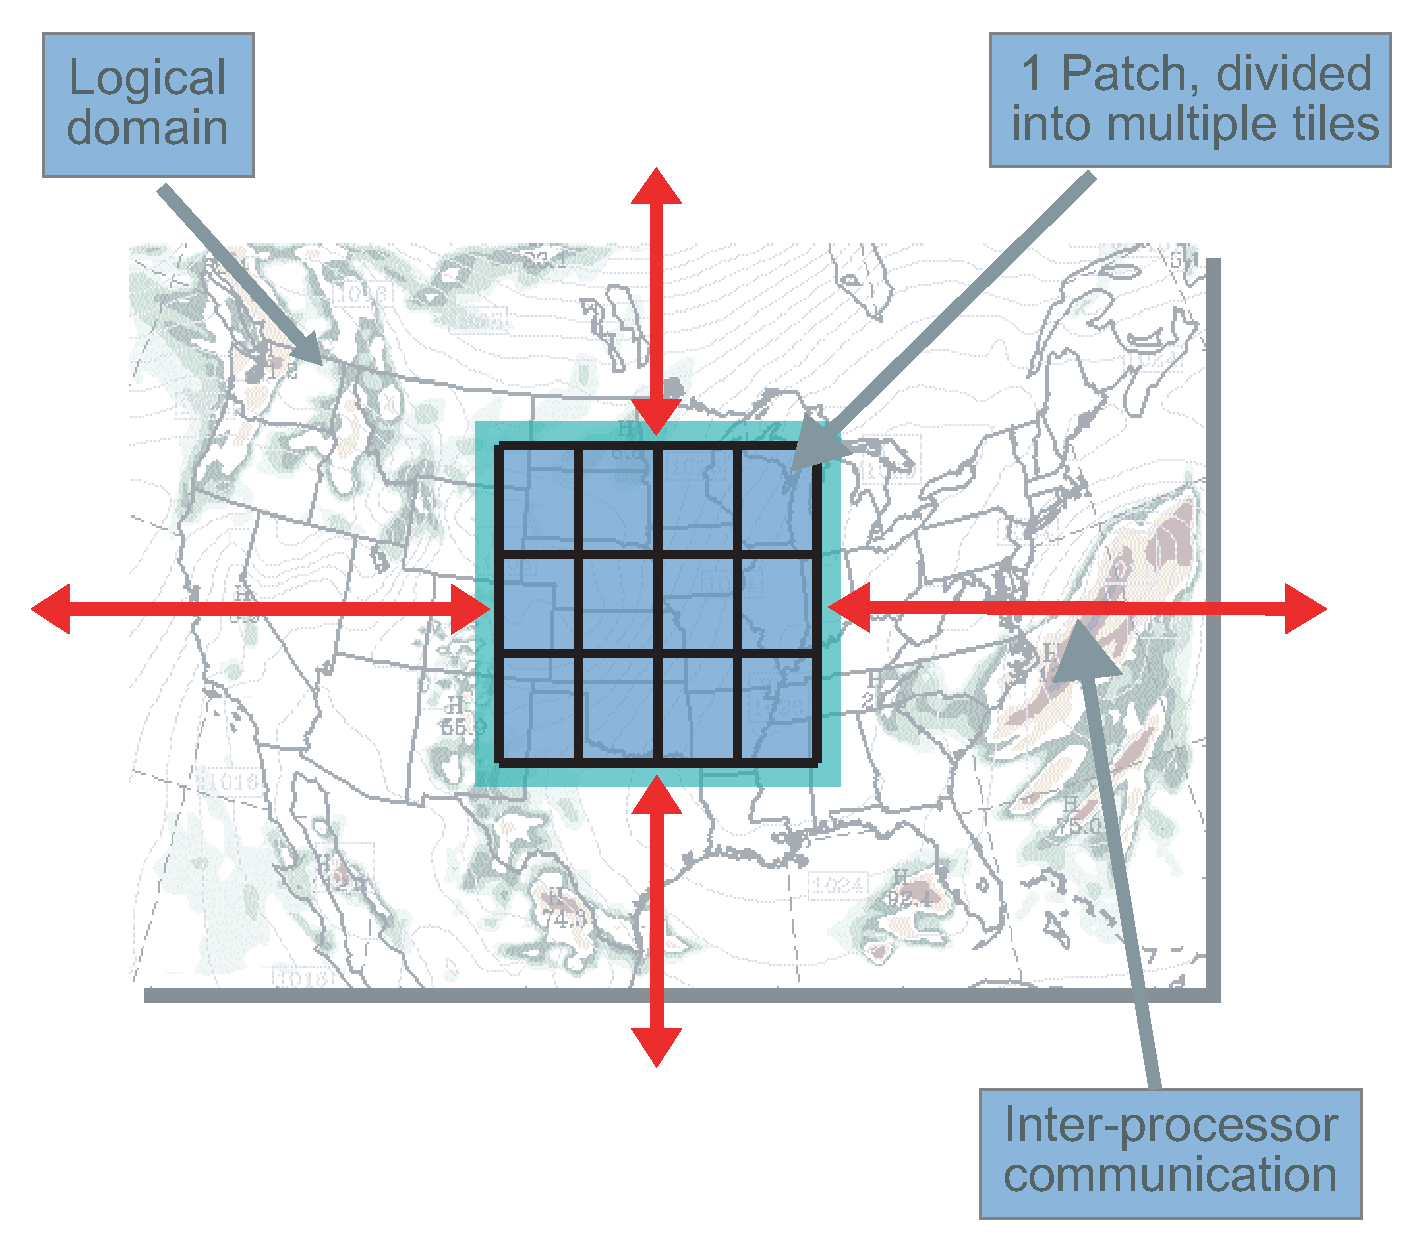
\includegraphics[width=6.5in]{figures/tile_patch.pdf}
  \caption{\label{figure:decomposition}Two-level horizontal domain decomposition, first over patches assigned to
distributed memory processes (only one shown). Patches then further subdivided over tiles, assigned to shared-memory threads
within each process.}
\end{figure}
\fi

\section{Nesting and Moving Nests}
\label{arch:2}

Nesting is the most complex
part of the WRF software.  Any domain may may be
parent to one or more nested domains, possibly with nests themselves, that can open, close, or move
at any time during the simulation.  Each
parent-nest pair exchanges data every parent time step for scores of model
variables, interpolated and masked in numerous different ways depending
on the field.  The entire model solution must consistently advanced
forward in time so that, at the end of each step, the entire hierarchy
of nested domains is at the same time-level.  A considerable part of
the WRF ASF design and implementation is devoted to supporting these
capabilities efficiently and on large numbers of parallel processes.
The ASF supports dynamic
configuration, instantiation, initialization, and movement of nests
according to dynamic aspects of a running simulation and to arbitrary
levels of refinement within the limits of machine resources. It manages
state data field sets on each domain according to how these participate
in nest initialization, forcing, and feedback with built-in or
user-supplied interpolators and masks applied on a field-by-field basis.
And it does so efficiently and scalably on large numbers of
processors.

The nesting hierarchy is a tree, rooted at the the top-most (most
coarse) domain.  Higher resolution nested domains are children of this
node that may, in turn, have child domains to the level of desired
refinement.  The driver level ASF represents this tree as a collection
of domain objects (instances of a Fortran 90 derived data type storing
the state fields for a given domain) that are linked together through
pointers, which represent the relationship of one domain to another.
Each domain has pointer to a parent (a nest may have only one; the top
level domain has no parent) and a number of pointers to domains that
are nests (if any) of this domain. Moving the nested simulation forward
is a matter of repeatedly traversing this tree-shaped network of domain
objects, once for each time-step on the coarse domain. The specific
strategy is a depth-first traversal of the tree -- that is, for a given
domain, the domain itself is first integrated forward one time step,
then the subtree rooted at the domain pointed to by this domain's child
pointer(s) integrate forward a series of smaller steps, bringing them
to the same time level as the current domain.  The algorithm is
naturally recursive, and the WRF ASF implements it that way: the routine
in the WRF ASF that integrates a domain forward to a given time-level
calls itself to do the same thing for each child.  This type of
recursion 
became part of the standard beginning with
Fortran 90.

Efficient and scalable implementation of nesting is a key concern. All
domains in a nested simulation are decomposed over the same set of
processes and nested domains run synchronously with the parent.
Exchanging forcing and feedback information requires communication to
scatter and gather data across processes at every parent time step. In
addition, interpolation of parent domain data to nest points is load
imbalanced because it only occurs over regions of the domain shared by
both parent and nest. This is partially alleviated by first rearranging
the parent domain data to the processes storing the corresponding nest
domain points, allowing interpolation to be performed locally and over
a larger number of processes.  The yellow region of Figure
\ref{figure:5} shows a lower-resolution parent domain decomposed over
24 distributed memory patches, each assigned to an MPI task.  The green
region inside represents the part of the parent domain that overlays
the higher-resolution nested or child domain. The decomposition of the
child domain is not shown, but it is also divided into 24 distributed
memory patches that are assigned to the same set of MPI tasks as the
parent domain. Each MPI task first advances the solution of its
parent-domain patch forward one time step. Then, MPI tasks that have
patches of the coarse domain that overlay the nested domain boundary
(for example, `a' and `b' in the figure) scatter that parent domain
data; that is, they send messages (black arrows going outward) to the
MPI processes that are responsible for patches of the child domain that
contain the child domain's boundary (for example, `c' in the figure).
The receiving processes store this parent domain data onto patches of
an intermediate domain: a domain that is at the lower-resolution of the
parent domain, but that is decomposed the same way as the corresponding
patch of the nested domain (upper-right of figure).
From this point forward the interpolation from parent to child
resolution is a local computation on each process that has a patch
containing the nest boundary.  Interpolating on the nested
decomposition is also more efficient, because more processors are
involved than if the interpolation were computed on the smaller number
of processes that overlay the nested boundary region.

%
% Figure 9.1
%
\ifnum\count33<9
\begin{figure}
  \centering
  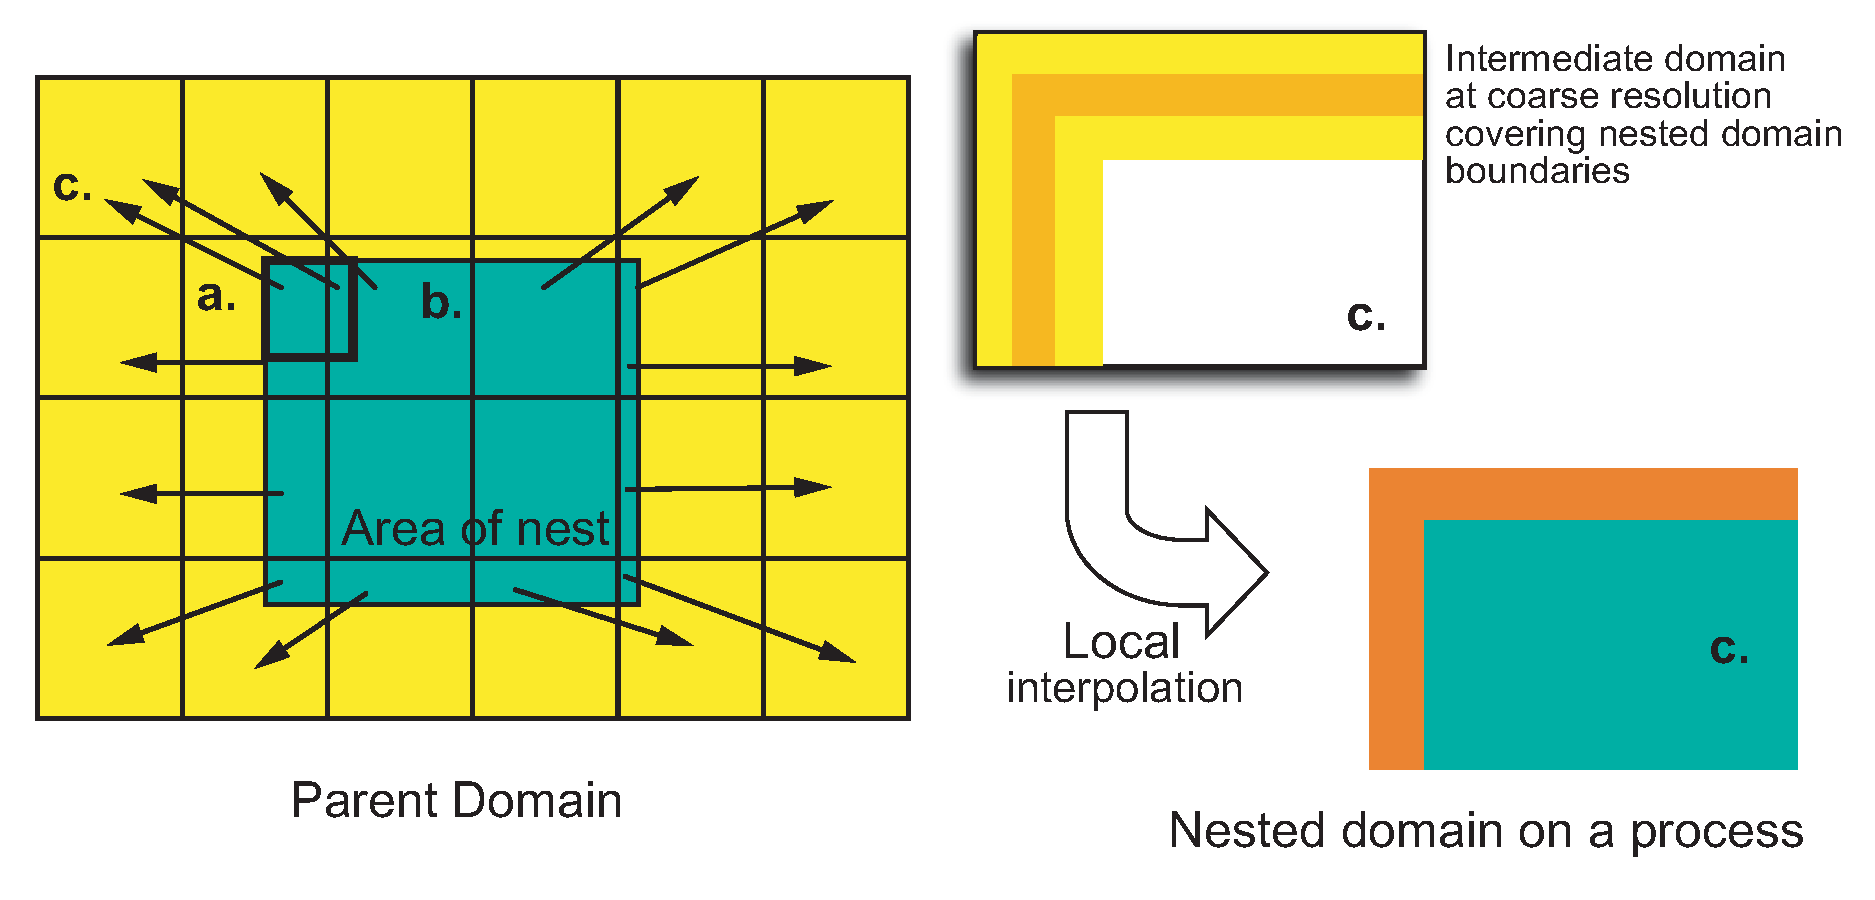
\includegraphics[width=6.5in]{figures/asf-nesting.pdf}
  \caption{\label{figure:5}Nesting decomposition and communication.}
\end{figure}
\fi

Nesting overhead has been measured by running equally dimensioned parent and 
nest domains as two-way interacting domains and then separately as stand-alone 
single domain runs. Overhead for nesting is between 5 and 8 percent, depending on 
the number of processes, and well within the target of 15 percent overhead observed 
in the parallel MM5 model. Most of the overhead appears related to the cost of the 
interpolation, which uses a relatively expensive non-linear algorithm.
The approach for moving nests is the same as two-way nesting, with some additional 
logic added to the framework and the model code:

\begin{enumerate}\setlength{\parskip}{-4pt}
  \item Determine whether it is time for a move and, if so, the direction and distance of the move. 

  \item Adjust the relationship between points on the nest and corresponding points on the parent domain.

  \item Shift data in the 2- and 3-dimensional state arrays of the nest in the opposite direction of the nest movement.

  \item Initialize the leading edge of the nest as it moves into a new position relative to the parent domain. Additional work is needed in step 1, above, to incorporate an automatic feature-following 
nest movement mechanism and in step 4 to allow run-time ingest of nest-resolution lower 
boundary data such as topography and land use on the leading edge of the moved nest. 

  \item The issue of coupling a moving domain to an external model such as an ocean model will be addressed in a later release.
\end{enumerate}

\section{I/O and Model Coupling}

The I/O system within the WRF ASF, like the ASF itself, is designed to
satisfy a hierarchy of requirements. 

For users of the model, the I/O system is presented at a high
domain-level as configurable streams that perform an I/O operation
on an entire domain. A domain-level input or output operation on a domain
results in a {\em frame} -- a set of state fields plus meta-data at the same
time-level -- being read from or written to a dataset on a stream.
The set of fields that make up a frame is configurable at compile-time
and is also easily controlled by the user through modifications to the
Registry (Section \ref{registry}).  There are streams for
primary and auxiliary {\em input}, primary and auxiliary {\em history}, {\em restart}, and
{\em boundary} data. All streams are bidirectional, the direction
depending on the application. The input stream is output by the real
data preprocessor. The WRF model may perform both input and output
on the input data stream, the output of which may serve as input to 3D-Var.
Data may be written in a number of different {\em formats}:
NetCDF, HDF, GRIB\footnote{Only GRIB edition output for now. GRIB edition 1 input and
GRIB edition 2 capabilities are in-progress.}, native binary, or through a
on-line model-coupling layer to another component model.  The dataset
name, format, times, and frequency of domain-level I/O on a given
stream are controlled at run-time via the program's namelist.  Streams
may be assigned different formats so that, for example, the model
model can be inputting NetCDF and outputting GRIB.

The domain-level layers of the ASF I/O system also manage parallel I/O;
that is the reading and distribution and the collection and writing of
data moving between undecomposed data sets and multiple
distributed-memory processes running the application.  In the case of
formats such as Parallel HDF5 that already support parallel I/O, the
ASF simply hands over the task of parallel I/O to the external package
implementing the format. In the case of other formats that do not
support parallel I/O, the ASF automatically collects and distributes
the data on one process before calling the package. The ASF also has
the ability to read and write input from decomposed data sets; that is,
each processor reads and writes its own file. This is useful for very
large model domains or for restart data sets, provided the model is
restarted using the same number of parallel processes. Finally, the ASF
supports an asynchronous output capability called $``$quilting$"$, the name
for which is borrowed from a similar capability in the NCEP operational
Eta model. The concept has been around in many earlier models including
the parallel implementation of MM5 and in the NOAA/Forecast Systems Laboratory parallel
implementation of the RUC model. One or more additional parallel
processes are used as I/O servers. When it is time to generate output,
processors responsible for model integration send their part of the
output to the servers, which then assemble and write the data to the
dataset while the compute processes continue with the model integration.

For developers and those working with other applications who wish to
use WRF I/O but at a level of I/O lower than on entire domains, there is
a lower-level WRF I/O and Model Coupling API.  The I/O and Model
Coupling API (I/O API, for short) within the WRF ASF provides a
uniform, package-independent interface between the WRF model and
external packages for I/O, data formatting, and coupling to other
models in larger multi-component simulations, for example, WRF coupled
with an ocean model.  A complete description and reference for the I/O
API is provided as an appendix to \citet{michalak03}. Implementations may
fully conform to the API or support as much functionality as they are
able.  The API specifies inquiry functions that return information
about the specific capabilities of an implementation.

Fully conforming implementations of the I/O API support complete
memory-order, transparency and provide random access to fields.
Memory-order transparency means that any application can access a
dataset through the I/O API, simply by providing the API with a
description of the application's internal memory order for the field
being accessed. Transposition of the data between the dataset and the
application's memory storage order is automatic and transparent. For
example, the WRF model stores three dimensional arrays in I-K-J memory
order; the 3D-Var program stores them as I-J-K.  Yet each is able to
access the same datasets through the WRF I/O API.  Fully conforming
implementations of the I/O API are also precision-transparent: the WRF
model and 3D-Var systems are able to share datasets even though 3DVAR
uses double-precision (64-bit) floating point precision while the model
typically uses single-precision (32-bit).  Random access means that a
field in a dataset is accessible by name and time-stamp only. Strictly
sequential access is also supported for performance or for
implementations, such as Fortran unformatted sequential I/O, that do not
support random access.

File I/O implementations of
the API for NetCDF, Parallel HDF5, native-binary, and GriB1 I/O are
run-time assignable to the framework's I/O streams.  The first
implementation of the I/O API, in NetCDF was developed by Jacques
Middlecoff at NOAA/FSL. Later, parallel HDF5 (Kent Yang, NCSA) and
GRIB1 (Todd Hutchinson, WSI) implementations were added to WRF as
contributed code from the user community.

The WRF I/O API also
supports model coupling, an idea well developed under \citet{coats99}
and in the PRISM coupling framework \citep{guilyardi02}.  Coupling as
I/O is attractive in that it allows encapsulation of details of
component data exchange within a model's control structures and
interfaces that already exist for I/O.  This method of coupling requires little if any
modification to the models, is readily and efficiently
adaptable to different forms of coupling (sequential or concurrent), 
can switch transparently (from the application's point of view) between
on-line and off-line modes of coupling, and is naturally suited to
distributed computing environments such as Grid computing.

Two model coupling implementations of the WRF I/O and Model Coupling
API have been developed: the Model Coupling Toolkit (MCT)
\citep{larson01} is the basis for the Community Climate System Model
(CCSM) coupler; the Model Coupling Environment Library (MCEL)
\citep{bettencourt02} is a CORBA-based client-server based coupling
framework.

The MCT implementation of the WRF I/O and Model Coupling API supports
regular, scheduled exchanges of boundary conditions for tightly to
moderately coupled interactions between WRF and the Regional Ocean
Modeling System (ROMS).  WRF wind stress and heat fluxes are sent to
the ocean model and sea-surface temperature is received from ROMS.
Three performance benchmarks of the WRF/ROMS coupling were conducted
and coupling overhead was nominal, well under 1 percent of total run
time for the coupled system. The coupled WRF/ROMS system has been used
in follow-on scientific studies involving an idealized hurricane vortex
described in \citet{nolan02}. The WRF/ROMS MCT implementation has been
demonstrated using the MPICH-G2 library within the Globus toolkit over
a rudimentary computational grid.  ROMS ran on one Intel Linux node at
NOAA Pacific Marine Environmental Laboratory (PMEL) in Seattle; WRF on
four Linux nodes at NOAA Forecast Systems Laboratory (FSL) in Boulder.
Even over geographically distributed systems, overhead for the WRF/ROMS
coupling using MCT over Globus was less than 2 percent.

The MCEL implementation of the WRF I/O and Model Coupling API supports
coupling of sets of models with a wider range of spatial and temporal
scales, or with irregular, data-driven interactions. Figure
\ref{figure:6} shows output from a four-model simulation of the Yellow
Sea littoral environment for a high-wind event in November, 1999. WRF
is coupled to a system composed of the ADCIRC ocean and SWAN wave
models.  ADCIRC and SWAN, in turn, provide forcing to a sedimentation
and optics model that simulates diver visibility \citep{allard02}.
ADCIRC, which uses an unstructured mesh, was also interfaced to MCEL
through the WRF I/O API in order to demonstrate its applicability to
other models and grid systems. MCEL supports concurrent coupling,
meaning that the components run at the same time on different sets of
processors.  Figure \ref{figure:7} shows the timing of interactions
between the components. As with MCT, the measured coupling overheads
were small.  WRF, the atmosphere, is the dominant cost of the
simulation.  Therefore, we measured the coupling overhead from the
point of view of the WRF model run. The cost of coupling measured from
WRF is only 15-20 milliseconds per exchange in each direction. With WRF
running on 4 processors, the coupling overhead is negligible, less than half
a percent of total run time. On 32 processors, the overhead from
coupling is under 5 percent of the cost of the run.

%
% Figure 9.2
%
\ifnum\count33<9
\begin{figure} 
  \centering
  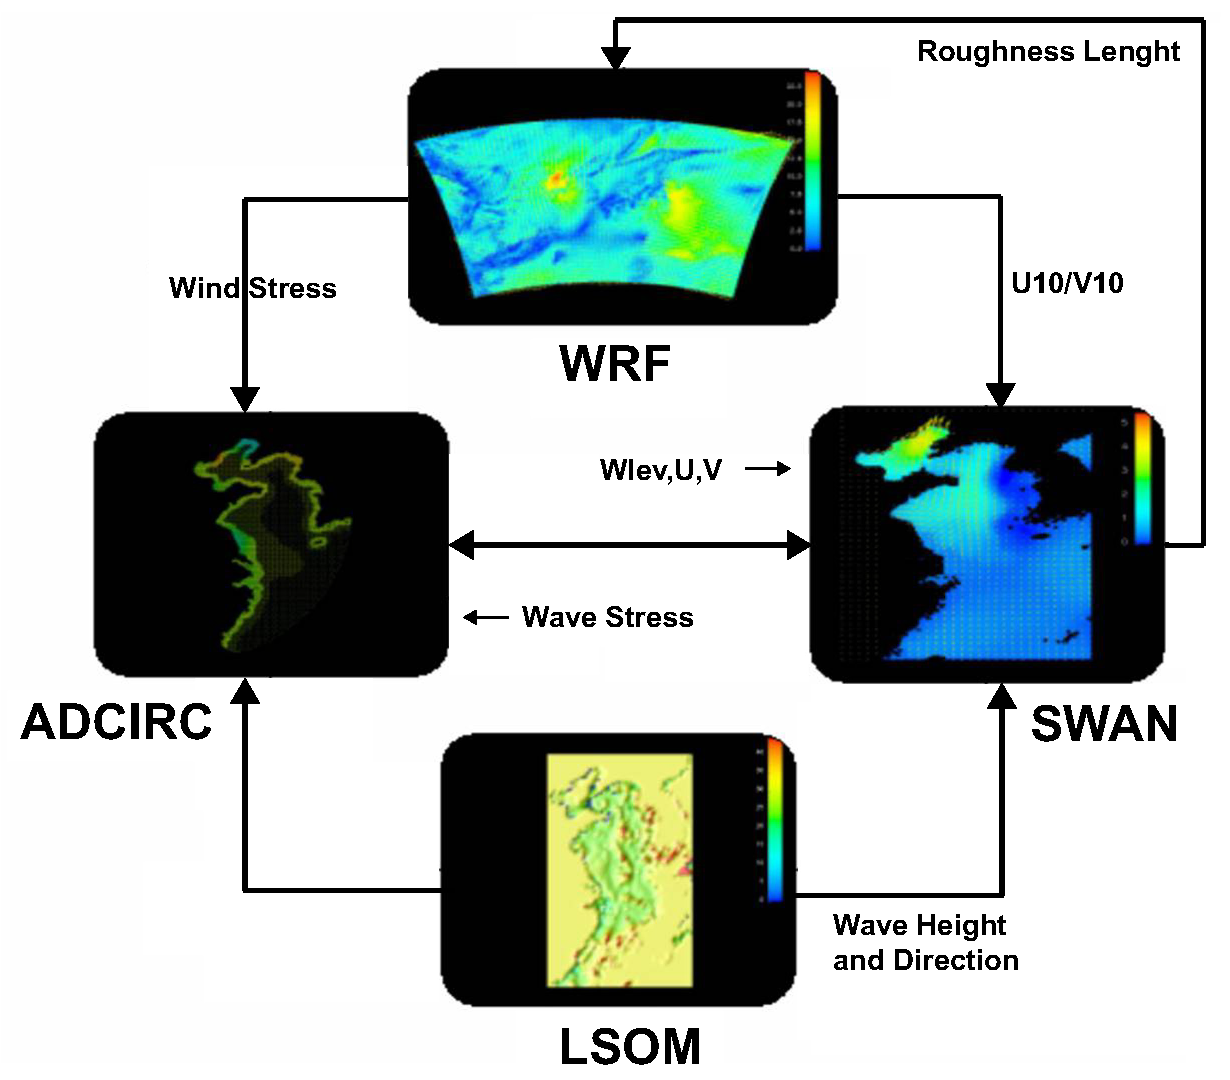
\includegraphics[width=6in]{figures/coupling.pdf}
  \caption{\label{figure:6}Coupling graph for Yellow Sea simulation showing WRF (atmosphere),
           ADCIRC (ocean circulation), SWAN (wave model), and LSOM (sediment optics).}
\end{figure}
\fi

The Earth System Modeling Framework, an emerging community-based standard 
and software infrastructure employs a different approach to model coupling. As 
opposed to handling coupling as a form of I/O, ESMF components are restructured 
to conform to a top-level ESMF-compliant component interface. This allows an 
ESMF-based driver to control model initialization, integration, and finalization. 
Coupling data are exchanged between components by passing import and export 
state objects through the components top-level interface.  Multi-executable mode
and compatibility with distributed and Grid-computing environments are
not currently supported.

%
% Figure 9.3
%
\ifnum\count33<9
\begin{figure}
  \centering
  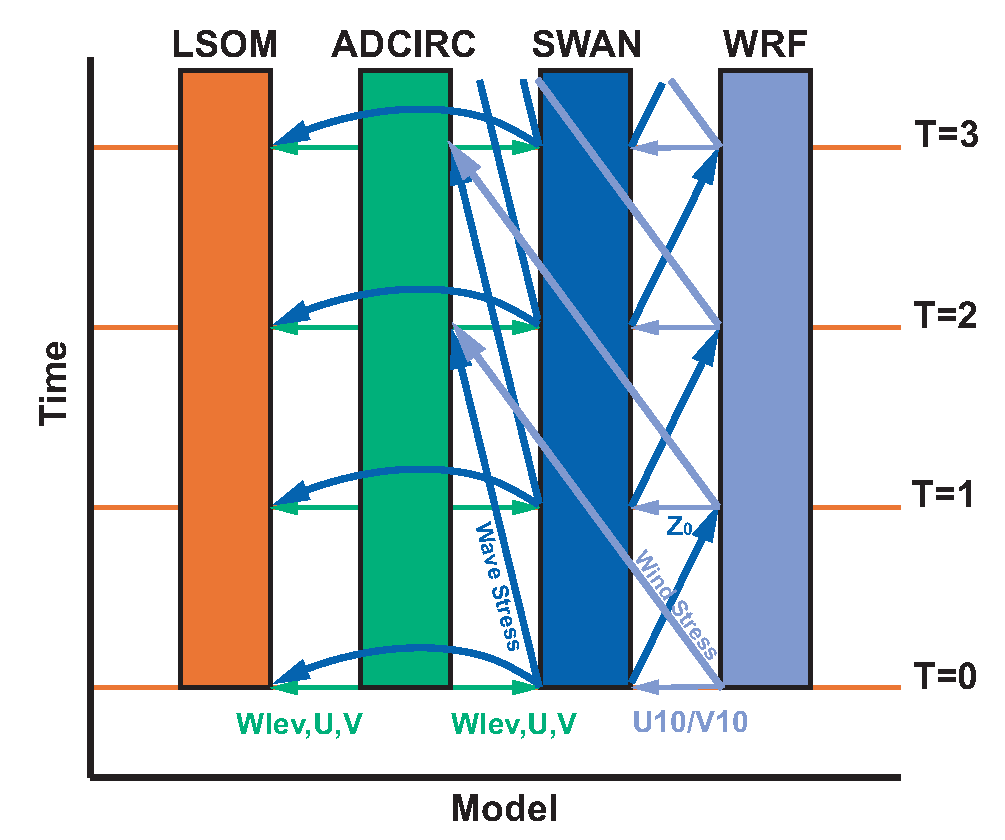
\includegraphics[width=4in]{figures/coupling2.pdf}
  \caption{\label{figure:7}Schedule of data interaction between four concurrently executing
           models. The coupling interval, T, is one hour.}
\end{figure}
\fi

WRF is being adapted to support top-level interface requirements to
interoperate as an ESMF coupled component but will also continue to
interoperate through I/O-like coupling mechanisms through the WRF I/O
and Model Coupling API. Implementing a form of ESMF coupling that
presents itself through the WRF I/O and Model Coupling API is also
being explored.

\section{Performance}

%
% Figure 9.x
%
\ifnum\count33<9
\begin{figure}
  \centering
  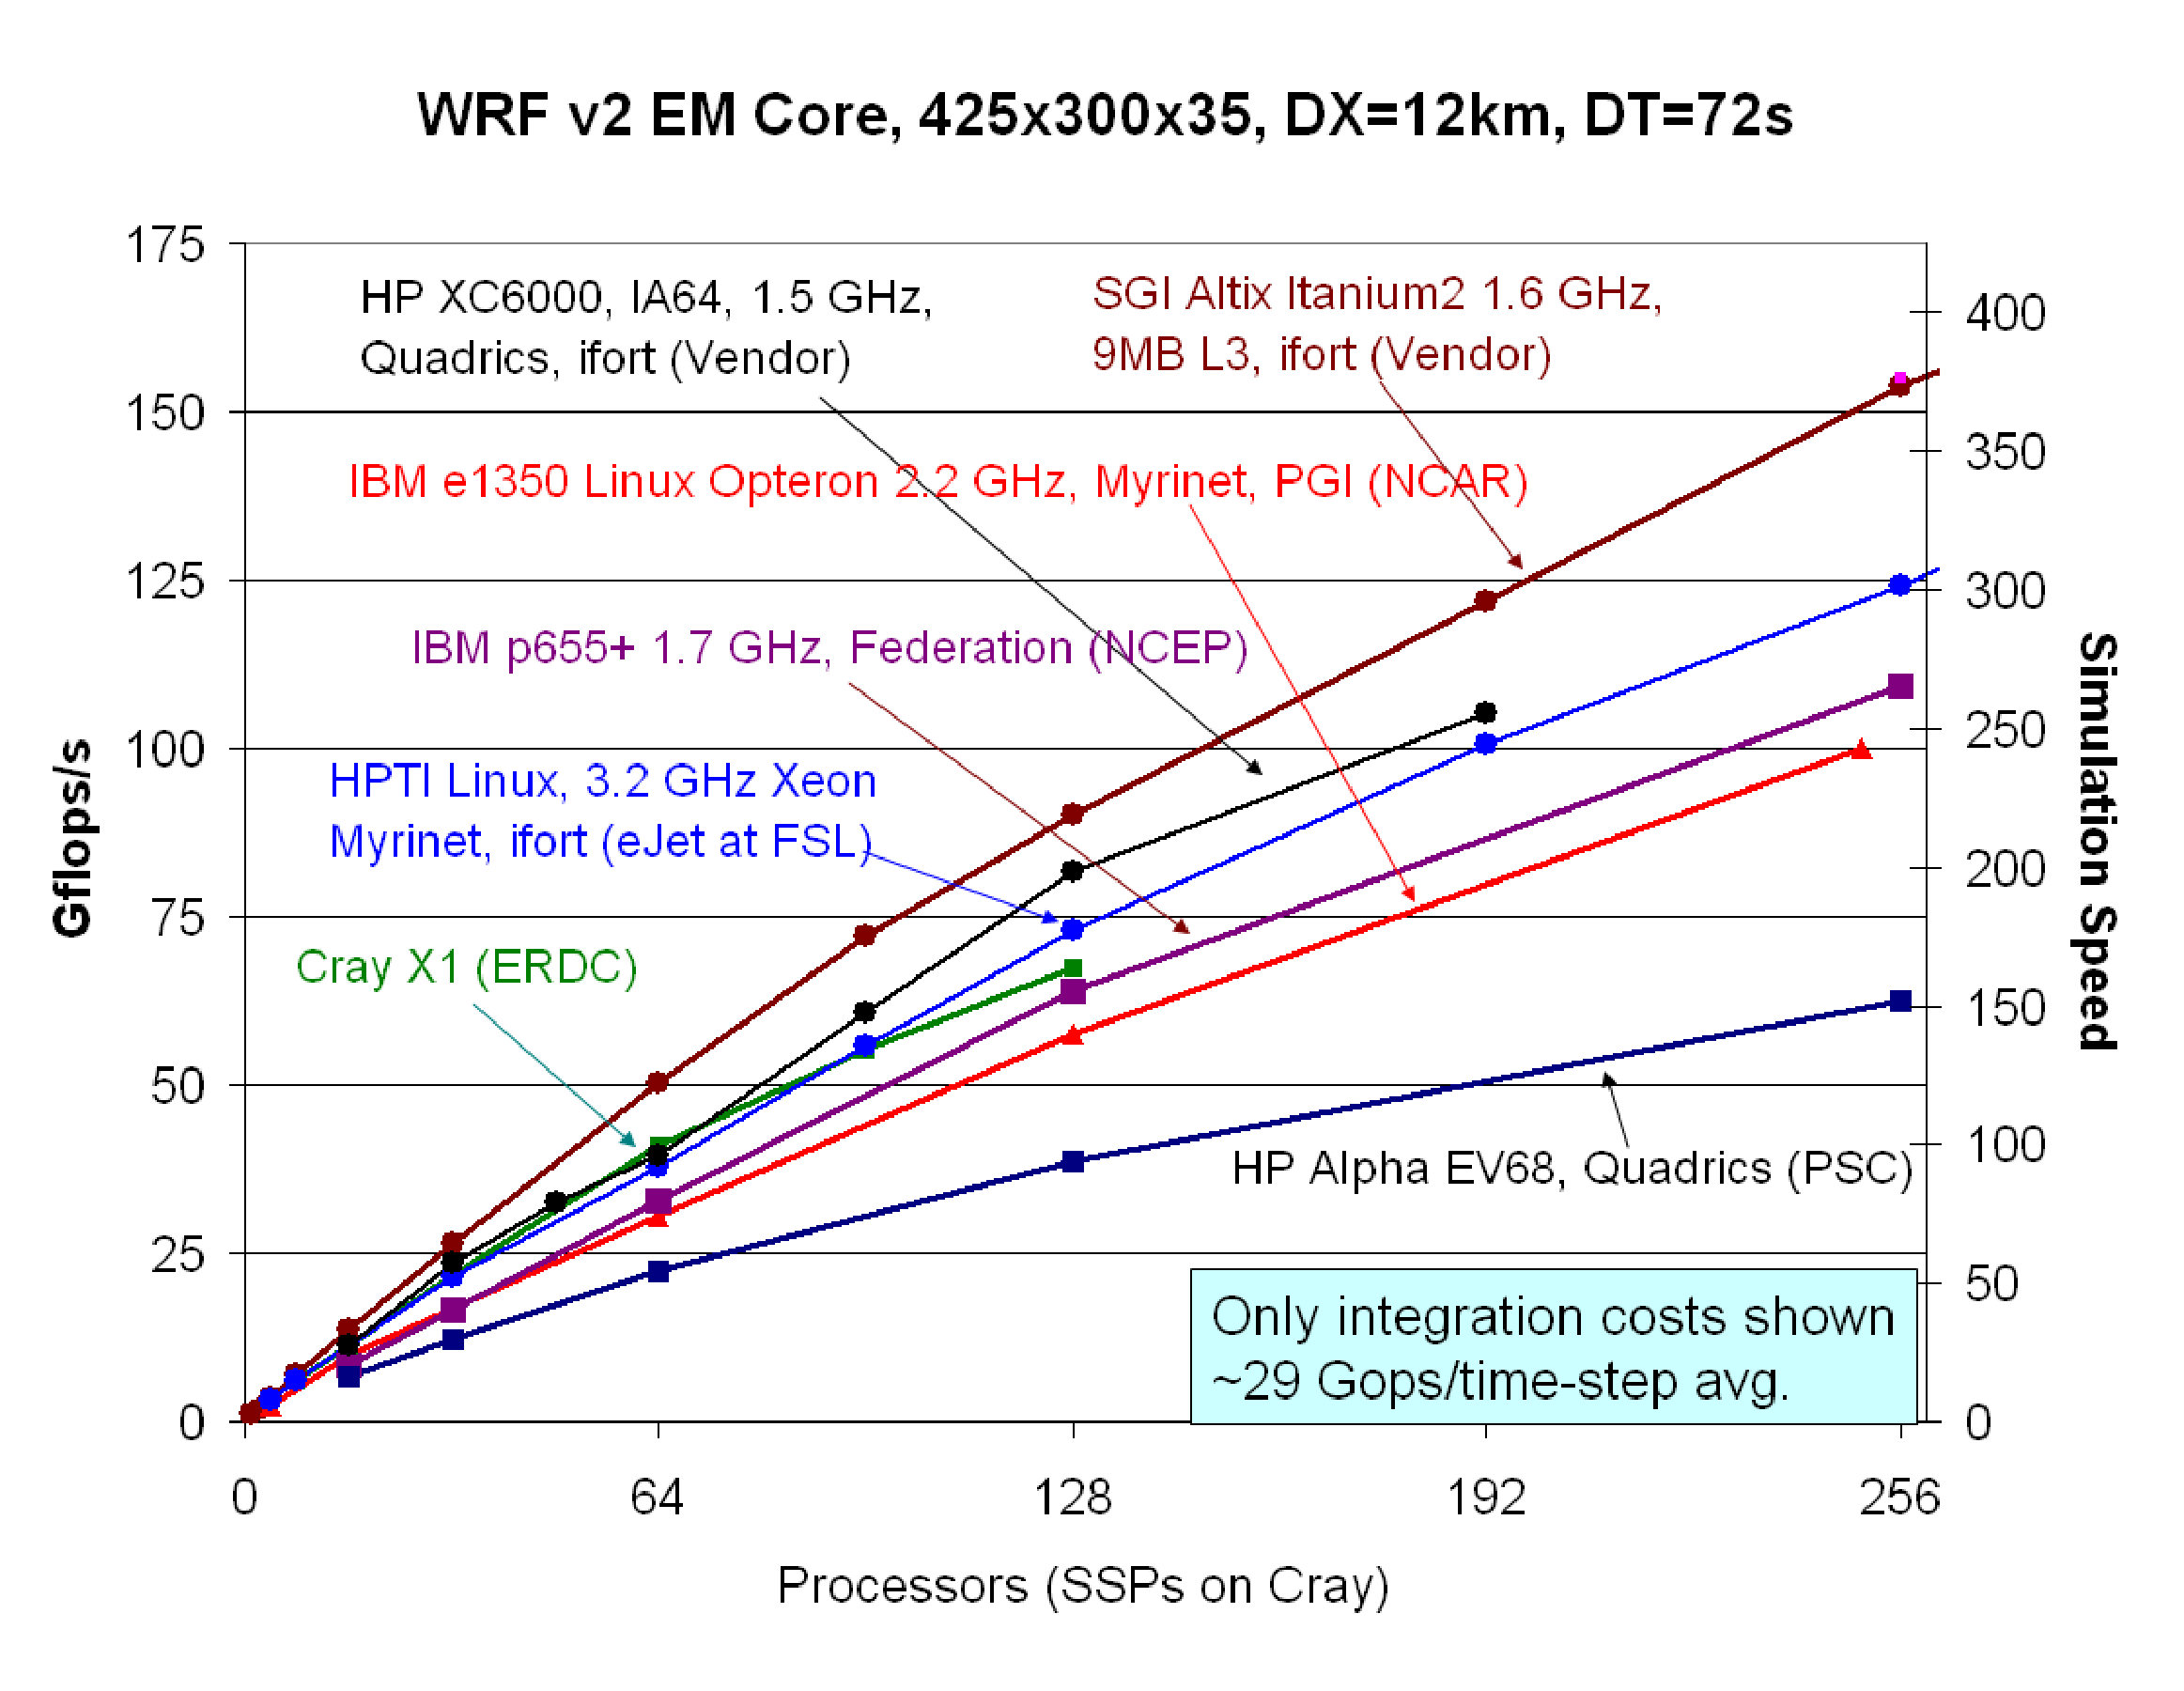
\includegraphics[width=5in]{figures/performance.pdf}
  \caption{\label{figure:performance} WRF Performance, Spring 2005.}
\end{figure}
\fi

Key goals for the WRF software are portability and efficiency over
shared, distributed-memory, and hybrid parallel architectures and over
both vector and scalar processor types. The WRF ASF supports a
two-level decomposition strategy that first decomposes each model
domain over distributed-memory patches and then, within each patch,
over shared-memory tiles. The framework and the Model Layer Interface
allow the Driver layer to decompose domains over arbitrarily shaped and
sized rectangular patches and tiles, giving maximum flexibility for
structuring the computation as efficiently as possible. Towards the
goal of WRF performance-portability, routine benchmarking on a variety
of target computer platforms has been ongoing.

The test case in Figure \ref{figure:performance} is a 48-hour, 12km resolution
case over the Continental U.S. (CONUS) domain.  The computational cost
for this domain is about 29 billion floating point operations per
average time step (72 seconds). Performance is defined as model speed,
ignoring I/O and initialization cost, directly measured as the average
cost per time step over a representative period of model integration,
and is presented both as a normalized floating-point rate and as
simulation speed. These are equivalent measures of speed, but
floating-point rate expresses speed as a measure of efficiency relative
to the theoretical peak capability while simulation speed, the ratio of
model time simulated to actual time, is more relevant as a measure of
actual time-to-solution.

The purpose of this WRF benchmark is to demonstrate computational
performance and scaling of the WRF model on target architectures. The
benchmarks are intended to provide a means for comparing the
performance of different architectures and for comparing WRF
computational performance and scaling with other similar models.  In
light of the continuing evolution and increasing diversity of
high-performance computing hardware it is important to define what is
being counted as a process.  For this benchmark, a parallel process is
the finest-grained sequence of instructions and associated state that
produces a separable and disjoint part of the solution.  Typically, the
number of processes is the number of WRF tiles are executing in
parallel during a given run.
The latest performance results are maintained and routinely updated on
the web\footnote{http://www.mmm.ucar.edu/wrf/bench}.


